\documentclass[9pt,twoside]{pnas-new}

% Use the lineno option to display guide line numbers if required.
\usepackage{adjustbox}  % in preamble
\usepackage{booktabs}
\usepackage{multirow}
\usepackage{graphicx}
    
\usepackage{pdfpages}
\usepackage{amsmath}
\usepackage{amsthm}
\usepackage{amssymb}
\usepackage{setspace}
\usepackage{graphicx}
\usepackage{booktabs}
\usepackage{pdflscape}
\usepackage{url}
\usepackage{caption}
\usepackage{multirow,rotating,multicol}
\usepackage{listings}
\usepackage{longtable}
\usepackage{threeparttable}
%\usepackage[position=top, font=normalsize]{subfig}
\usepackage{subcaption}
\usepackage{float}
\usepackage{pgfpages,tikz}
\usepackage{adjustbox}
\usepackage{enumitem}
\usepackage{appendix}
\usepackage{dsfont}
\usepackage{natbib}
\usepackage{bookmark}

% Captions and notes in the body font (Latin Modern Roman) instead of the
% class's sans-serif caption format; table captions keep their bold label.
\DeclareCaptionFormat{rmformat}{\normalfont\rmfamily\footnotesize#1#2#3}
\captionsetup*{format=rmformat}
\captionsetup*[figure]{labelfont={bf}}
\captionsetup*[table]{labelfont={bf},textfont={rm},skip=6pt,position=above}

\templatetype{pnassupportinginfo}


\title{Beyond Stoves and Outdoor Monitors: Indoor PM2.5 Concentrations and Inequality in a Fast Growing Megacity}

% Use letters for affiliations, numbers to show equal authorship (if applicable) and to indicate the corresponding author

% \title{Your main manuscript title}
\author{Sun, Sorin, Suryadarma, Rahut and Resosudarmo}
\correspondingauthor{Sorin \\E-mail: jsorin@berkeley.edu}

\begin{document}
\pagestyle{plain}
\fancyhf{}
\maketitle

\renewcommand{\thefigure}{S\arabic{figure}}
\renewcommand{\thetable}{S\arabic{table}}


%% Adds the main heading for the SI text. Comment out this line if you do not have any supporting information text.
% \SItext


% \subsection*{Subhead}
% Type or paste text here. This should be additional explanatory text such as an extended technical description of results, full details of mathematical models, etc.   

% \section*{Heading}
% \subsection*{Subhead}
% Type or paste text here. You may break this section up into subheads as needed (e.g., one section on ``Materials'' and one on ``Methods'').

% \subsection*{Materials}
% Add a materials subsection if you need to.

% \subsection*{Methods}
% Add a methods subsection if you need to.
\newpage


\SItext
\begin{adjustwidth}{1cm}{1cm} 
\section*{Survey Instruments}

\subsection*{Baseline Survey Instruments}

Study participants were asked the following survey questions during a baseline survey, before the installation of the air quality monitoring hardware.\footnote{These questions were part of a longer survey.} Bahasa Indonesian translations are in parentheses.

\begin{enumerate}
\item What was your household's total income in the past month (in IDR)? This includes cash transfers from the government (\textit{Berapa penghasilan rumah tangga dalam sebulan terakhir? (dalam Rupiah)})
\begin{enumerate}
    \item $<$Rp 1.000.000
    \item Rp 1.000.000 - Rp 2.999.999
    \item Rp 3.000.000 - Rp 4.999.999
    \item Rp 5.000.000-Rp 7.999.999
    \item Rp 8.000.000 - Rp 9.999.999
    \item Rp 10.000.000 - Rp12.999.999
    \item $>$13.000.000
        \item Does not know (\textit{Tidak tahu})
        \item Refuse to answer (\textit{Menolak menjawab})
\end{enumerate}
\item How many rooms does this residence have? (\textit{Berapa banyak kamar yang dimiliki hunian ini?})

[Enumerator: Count spaces as separate rooms only if they have a formal entrance, even if the door is a curtain. Do not count one room divided by curtains without a formal entrance as separate rooms. Family-owned shops attached to the residence and bathrooms should count as rooms.] \\ 
(\textit{[Enumerator: ruangan dianggap terpisah jika ada tempat masuk, meskipun pintunya adalah kain. Jika tidak ada tempat masuk, meski terpisah oleh kain/gorden, jangan dihitung sebagai ruangan terpisah. Toko yang bersatu dengan rumah, kamar mandi, dihitung sebagai satu ruangan terpisah.]})

    \item In the past 7 days, how do you think air quality was in your home, on the scale we mentioned earlier? (\textit{Dalam seminggu terakhir, berdasarkan skala yang sudah saya sebutkan tadi, menurut Ibu/Bapak seberapa baik kualitas udara di Jakarta?})

    \begin{enumerate}
        \item Good (green) (\textit{Baik (hijau)})
        \item Moderate (yellow) (\textit{Sedang (kuning)})
        \item Unhealthy for sensitive groups (orange) (\textit{Tidak sehat untuk kelompok rentan (oranye)})
        \item Unhealthy (red) (\textit{Tidak sehat (merah)})
        \item Very unhealthy (purple) (\textit{Sangat tidak sehat (ungu)})
        \item Hazardous (Brown) (\textit{Berbahaya (coklat)})
        \item Doesn't know (\textit{Tidak tahu})
    \end{enumerate}

    
    \item Is there an air conditioner in the house? (\textit{Apakah terdapat AC/pendingin udara di dalam rumah?})
    \begin{enumerate}
        \item No (\textit{Tidak})
        \item Yes, in room the hardware is in (\textit{Ya, di ruangan yang terdapat air purifier dan air monitor})
        \item Yes, in another room in the house (\textit{Ya, di ruangan lain})
    \end{enumerate}
     
    \item In the past 7 days, how many times did you see trash being burned in your neighborhood? (\textit{Dalam seminggu terakhir, berapa kali Ibu/Bapak melihat sampah dibakar di lingkungan Ibu/Bapak?})
    \begin{enumerate}
        \item Never (\textit{Tidak pernah})
        \item 1 or 2 times (\textit{1-2 kali})
        \item 3 or more times (\textit{3 kali atau lebih})
        \item Does not know (\textit{Tidak tahu})
        \item Refuse to answer (\textit{Menolak menjawab})
    \end{enumerate}
    \item What is the main cooking fuel you use in your home? (\textit{Apa bahan bakar utama untuk memasak yang Ibu/Bapak gunakan di rumah?})
    \begin{enumerate}
        \item Electric (\textit{Kompor listrik})
        \item Gas/LPG (\textit{LPG})
        \item Kerosene (\textit{Minyak tanah})
        \item Charcoal/briquettes/coconut shells (\textit{Arang/briket/batok kelapa})
        \item Firewood (\textit{Kayu bakar})
        \item Other (\textit{Lainnya})
    \end{enumerate}

    
    \item I have a list of activities that could cause air pollution in the room the hardware is set up in. Can you verify if any of the following occur in the room of the purifier? (\textit{Saya memiliki daftar aktivitas yang dapat menyebabkan polusi udara di ruangan tempat alat dipasang. Bisakah Ibu/Bapak memberitahu apakah terdapat aktivitas berikut yang terjadi di ruangan yang terdapat air purifier?})
    \begin{enumerate}
        \item Gaps in doors and windows (\textit{Celah di pintu dan udara})
        \item Doors/windows are always open (\textit{Pintu/jendela yang selalu terbuka})
        \item Close to kitchen (\textit{Dekat dengan dapur})
        \item Smoking/vaping in or near the room (\textit{Merokok/vaping di dalam/dekat ruangan})
        \item Whether the room has doors and is connected to another room (\textit{Ruangan memiliki pintu yang terhubung dengan ruangan lain})
        \item Garbage burning in the neighborhood (\textit{Pembakaran sampah di lingkungan sekitar})
        \item Candles/Incense (\textit{Difuser/Pelembab udara/humidifier})
        \item None
    \end{enumerate}

\end{enumerate}

\noindent The baseline survey included a time-use recall module covering the period from 4\,AM the previous day to 10\,AM on the interview day. For each contiguous activity block, the respondent identified the activity from a fixed set of mutually exclusive categories and reported the hour at which the block ended. The cooking indicator used in our main specification (\texttt{1[CookingHour]} in Equation~1) is constructed from the adult respondent's reported cooking hours.

\begin{enumerate}
\setcounter{enumi}{\value{your_last_question_number}}

\item We now want to ask you about your activities from 4\,AM the previous day to 10\,AM today, the interview day. An activity is anything you did during the day. Activities include both active tasks like socializing, preparing food, or eating, and quieter tasks like relaxing and sleeping. These questions are for research purposes only; if you do not feel comfortable, you are not required to answer. If you are comfortable, I will begin with your activity at 4\,AM yesterday. (\emph{Pada bagian ini, saya akan menanyakan aktivitas Ibu/Bapak sejak pukul 4 pagi kemarin hingga pukul 10 pagi hari ini. Aktivitas yang dimaksud merupakan apapun yang Ibu/Bapak lakukan sepanjang hari yang mencakup bersosialisasi, menyiapkan makanan, makan, bersantai, tidur, bekerja, dan hal lainnya. Pertanyaan-pertanyaan ini dimaksudkan semata-mata untuk tujuan penelitian, tetapi jika Ibu/Bapak merasa tidak nyaman untuk menjawab pertanyaan ini, Ibu/Bapak diperbolehkan untuk tidak menjawab.})

\item Repeated for each activity block, beginning at 4\,AM and continuing until the cumulative time reaches 24 hours:

At [previous block end time], what activity were you doing? Please select from the following: (\emph{Pada pukul [previous block end time], aktivitas apa yang Ibu/Bapak lakukan? Pilih aktivitas berikut:})
    \begin{enumerate}
        \item Inside own home --- awake (\emph{Di dalam rumah Ibu/Bapak sendiri --- Bangun/Terjaga})
        \item Inside own home --- asleep (\emph{Di dalam rumah Ibu/Bapak sendiri --- Tidur})
        \item Inside own home --- cooking (\emph{Di dalam rumah Ibu/Bapak sendiri --- Memasak})
        \item Work / school (\emph{Bekerja / sekolah})
        \item Outdoors, non-exercise (\emph{Di luar ruangan --- tidak ada hubungannya dengan olah raga})
        \item Commuting (\emph{Bepergian})
        \item Outside the home, in an indoor space (\emph{Di luar rumah, di ruang dalam ruangan})
    \end{enumerate}

\item What hour did you end this activity? (\emph{Pada pukul berapa Ibu/Bapak mengakhiri aktivitas ini?})

    \noindent [Enumerator: enter the end hour on a 24-hour clock (e.g., 1\,PM is entered as 13). The module repeats with question (2) above asking about the next activity block, until cumulative elapsed time reaches 24 hours. Automated checks flag totals below 24 or above 31 hours for revision.] (\emph{[Enumerator: catat jam berakhir dengan format 24 jam, misalnya pukul 1 siang dicatat sebagai 13. Modul akan terus diulang menanyakan aktivitas berikutnya hingga total waktu mencapai 24 jam. Sistem akan memberi peringatan jika total kurang dari 24 atau lebih dari 31 jam.]})

\end{enumerate}

\subsection*{Endline Survey Instruments}

Study participants were asked the following survey questions during an endline survey, after the air quality monitoring hardware had been installed for two to three months.\footnote{These questions were part of a longer survey.} Bahasa Indonesian translations are in parentheses.

\begin{enumerate}
    \item In the last 24 hours, did someone smoke inside your home?	(\textit{Dalam 24 jam terakhir, apakah seseorang merokok di dalam rumah Anda?})
    \begin{enumerate}
        \item Yes (\textit{Ya})
        \item No (\textit{Tidak})
         \item Does not know (\textit{Tidak tahu})
        \item Refuse to answer (\textit{Menolak menjawab})
    \end{enumerate}
    
\end{enumerate}

\subsection*{Whatsapp Survey}

Study participants were also asked high frequency questions via Whatsapp during the course of the study. In particular, they were asked about their window/door opening activities:
\begin{enumerate}
    \item In the last hour, was the door to the room where the air quality equipment is stored open to the outside? (\textit{Dalam 1 jam terakhir, apakah pintu di ruangan tempat menyimpan alat kualitas udara terbuka ke luar? (jika ada pintu yang terbuka ke luar ruangan)})
    \begin{enumerate}
        \item Yes (\textit{Ya})
        \item No (\textit{Tidak})
        \item There are no outside doors (\textit{Tiada pintu ke luar})
    \end{enumerate}
        \item In the last hour, was the window in the room where the air quality equipment is stored open to the outside? (\textit{Dalam 1 jam terakhir, apakah jendela di ruangan tempat menyimpan alat kualitas udara terbuka ke luar? (jika ada jendela yang terbuka ke luar ruangan)})
    \begin{enumerate}
        \item Yes (\textit{Ya})
        \item No (\textit{Tidak})
        \item There are no outside windows (\textit{Tak ada jendela luar})
    \end{enumerate}
\end{enumerate}

\clearpage

\newpage
\pagebreak 
\subsection*{Envelope Tightening: Back-of-the-envelope} %6

Following \citep{chen_review_2011}, in steady-state, indoor PM$_{2.5}$ concentrations $C_{in}$ can be expressed as a function of outdoor PM$_{2.5}$ concentrations $C_{out}$, the air exchange rate due to infiltration \textit{a}, the penetration factor \textit{P}, the particle deposition rate \textit{k} and the indoor-source strength by volume \textit{S}:
\begin{align*}
    C_{in} &= \frac{a P C_{out} +S}{a+k}.
\end{align*}
The coefficient $\beta$ estimated in Eq. (1)  can be shown to correspond to the infiltration factor $F_{inf} = \frac{a P}{a + k}$. For the central back-of-the-envelope calculation, we set $P = 1$ and $k = 0.5 h^{-1}$ and solve for the implied air exchange rate
\begin{align}
    a &= \frac{\hat{F}_{inf} k}{P - \hat{F}_{inf}}
\end{align}
Given $(a, P, k)$, we recover indoor-source strength by volume as the residual
\begin{align*}
    S &= (a + k) C_{in} - a P C_{out}.
\end{align*}
Robust range: we vary the deposition loss rate $k$ over $[0.2, 1.5]~(h^{-1})$ and the penetration factor $P$ over $[0.8, 1.0]$. We evaluate the four corner combinations $(k_{min}, P_{min}), (k_{min}, P_{max}), (k_{max}, P_{min}), (k_{max}, P_{max})$; for each we solve for the implied $a=\frac{\hat F_{inf}k}{P-\hat F_{inf}}$ and recompute $S=(C_{in}-\hat F_{inf}C_{out})(a+k)$.
\\

This model can be leveraged in a simple back-of-the-envelope calculation to assess the impact of interventions that reduce air exchange (targeting \textit{a}) or reduce particle penetration of incoming air (targeting \textit{P}) on indoor PM$_{2.5}$ concentrations. This latter calculation isolates the effect of changing \textit{P} alone, holding \textit{a} fixed. In practice, physical mechanisms that reduce \textit{P} may also reduce \textit{a}.
Table \ref{SI_BoE_table} reports the key inputs and main results of this calculation, split by income and smoking status.
\\

The back-of-the-envelope exercise suggests that reducing particle penetration (lowering $P$) mechanically decreases indoor PM$_{2.5}$ in all households—under the convention that $P$ applies only to outdoor-to-indoor particle entry—whereas weatherization (reducing $a$) can have ambiguous effects because it also limits dilution of indoor emissions. In our central calibration, weatherization increases indoor PM$_{2.5}$ in low-income households, and this conclusion is robust over the parameter range considered. In contrast, weatherization decreases concentrations in high-income non-smoking households throughout the robust range; for high-income smoking households, the effect remains small and can change sign over the robust range. Precisely quantifying the impacts of interventions that alter $a$ and $P$ would require stronger empirical identification of these parameters, which is beyond the scope of this paper.



\newpage

\subsection*{LMG $R^2$ Decomposition} 
To complement the mean contribution decomposition in the main text, we decompose the $R^2$ of Equation 1 across predictors using the Lindeman-Merenda-Gold (LMG) method \citep{lindeman_introduction_1980}. 
In multiple regressions, the contribution of a predictor to explained variance depends on which other predictors are already in the model, rendering simple sequential decompositions sensitive to arbitrary ordering choices. LMG resolves the attribution problem that arises under predictor correlation by averaging each predictor's marginal $R^2$ contribution over all possible orderings in which predictors could enter the model. This method thus provides a consistent decomposition of explained variance. We implement this using the \texttt{relaimpo} package in \texttt{R} \citep{gromping_relative_2006}. 
The ranking of sources by $R^2$ contribution is consistent with the mean contribution decomposition in the main text: outdoor ambient pollution accounts for the largest share, followed by household smoking and waste burning, with kitchen source, cooking hour, and distance to main road contributing minimally. For pollution spikes, smoking is by far the dominant contributor, while waste burning also contributes substantially.



\newpage 

\subsection*{Sensor Validation}

Indoor PM$_{2.5}$ is measured by a Cubic PM2008M sensor inside the indoor device, while outdoor PM$_{2.5}$ is measured by Plantower PMS5003 in the Airly network sensors. One concern is that low-cost optical sensors may differ in calibration, and their response could vary with humidity, temperature and particle characteristics. We provide evidence that these concerns do not significantly affect our results from two collocation exercises.

First, an Airly PMS5003 sensor was collocated with the US Embassy regulatory-grade monitor in Jakarta between May and July 2024 (Fig.~\ref{fig:sensor_validation}a). We estimated an hourly $R^2 = 0.90$, a slope of $1.06$ and an intercept of $2.9$. While the two sensors track each other closely, the Airly PMS5003 sensor reads on average 13\% higher than the US Embassy sensor. 

In the second collocation exercise, three indoor devices with Cubic PM2008M sensors were deployed side-by-side with an Airly PMS5003 outdoor sensor for two weeks in September 2026 (Fig.~\ref{fig:sensor_validation}b--c; $N = 349$ hours). The estimated hourly $R^2$ values ranged from $0.88$ to $0.90$. Although the indoor devices closely tracked the outdoor sensor, they reported concentrations approximately 10~$\mu g/m^3$ lower on average. This discrepancy was largely a constant offset across the observed ranges of outdoor PM concentrations (23--100~$\mu g/m^3$), relative humidity (49--94\%), and temperature (24--33$^\circ$C).

The offsets observed in the two collocation exercises likely arose for different reasons. In the first exercise, the positive offset of the outdoor PMS5003 sensor relative to the US Embassy monitor is consistent with documented overestimation by uncorrected Plantower sensors in tropical, humid settings \citep{hossain_performance_2025, Wulandari2024}. In the second exercise, we attribute the negative offset of the indoor sensors to their placement inside the device, whereas the outdoor sensor was directly exposed to ambient air.

We invert the two relationships to map the recorded series into reference-grade-monitor units: $O^{ref} = (O - 2.9)/1.06$ and $I^{ref} = \big((I - a)/b - 2.9\big)/1.06$ and re-estimate our main results on the converted series. This exercise offers suggestive evidence that our headline results are robust and, if anything, conservative. The re-estimated headline results are reported below.

\vspace{.3cm}
\textit{Infiltration factor.} The infiltration factor is essentially unchanged: 0.62 (95\% CI [0.45, 0.79]) against 0.59 in the main estimate (Fig.~2a, Sensor Adjusted). The conversion amounts to dividing indoor readings by $b = 0.96$, since the intercepts are absorbed by the fixed effects and the outdoor sensor's calibration rescales both sides of Eq. (1) equally. Because measurement error in the outdoor sensor may attenuate the calibration slope, we also estimate the relationship with outdoor readings as the outcome and indoor readings as the predictor. Inverting the resulting slopes yields values of 1.0--1.2 and implies an adjusted infiltration factor of 0.50--0.59.

\textit{Concentration levels.} The estimated offset implies that recorded indoor levels are conservative. Assuming that the offset also holds below the collocated range would imply that mean indoor PM$_{2.5}$ is about 47.5 rather than 42.3~$\mu g/m^3$, the ratio of mean indoor to mean outdoor PM$_{2.5}$ increases to 1.37 rather than 1.07, the share of household-days above the WHO 24-hour guideline rises from 78\% to 88\%, and the share of households exceeding the guideline on at least one day rises from 97\% to 99\%. The exact figures depend on how the outdoor sensor's overestimation at low concentrations is modeled.

\textit{Source contributions.} Source effects in $\mu g/m^3$ (for example, the smoking effect) and comparisons across households (for example, the income gradient) are differences between indoor readings, in which a constant offset cancels. The source shares are affected because correcting the offset increases the estimated mean indoor PM$_{2.5}$ concentration, while leaving source-specific differences largely unchanged. Recomputing these shares using the adjusted readings, the outdoor share falls from 56\% to about 45\% and the smoking share from 19\% to about 17\%, with the remainder attributed to the baseline (intercept) component. The ranking of sources is unchanged, and ambient outdoor PM$_{2.5}$ remains by far the largest contributor.





\newpage
\section*{Figures}



\begin{figure}[!htb] %4
    \centering
    \caption{Infiltration Factor with Lagged Outdoor $PM_{2.5}$} 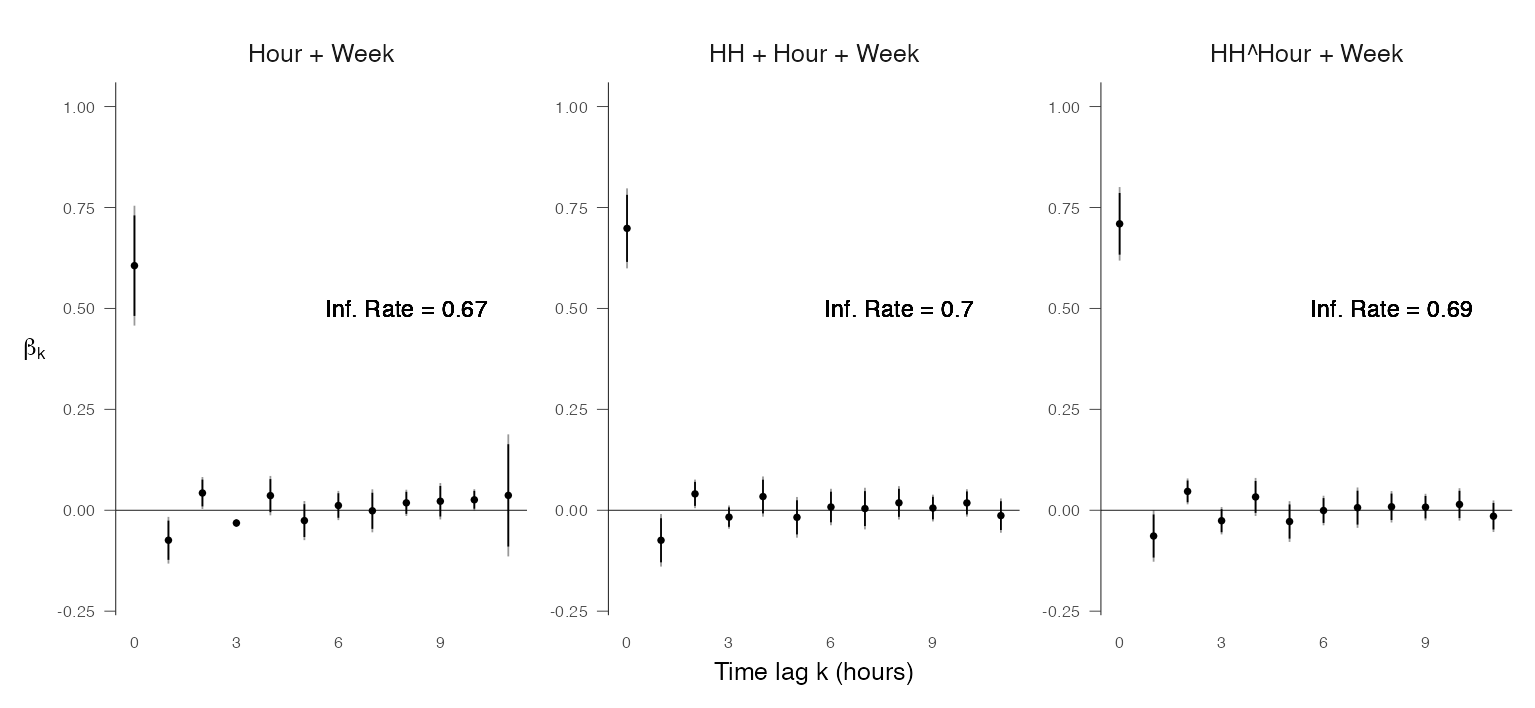
\includegraphics[width=.8\linewidth]{output_clean/figures/inf_lags.png}
    \caption*{\footnotesize Notes: Infiltration factor, showing the relationship between changes in outdoor concentration and changes in indoor concentrations. This shows the lags in the previous 11 hours. The model controls for hyperlocal source variables (waste burning frequency, household smoking, kitchen source presence, cooking activity, and distance to main road), outdoor temperature, humidity, and hour-of-day and week fixed effects. Points represent mean estimates; darker error bars show 90\% confidence intervals, and lighter error bars show 95\% confidence intervals. Errors are clustered at the household level. }
    \label{fig:inf_lag}
\end{figure}

\clearpage


\pagebreak
\begin{figure}[!htb] %1
    \centering
    \caption{Missing Indoor PM$_{2.5}$  Data} 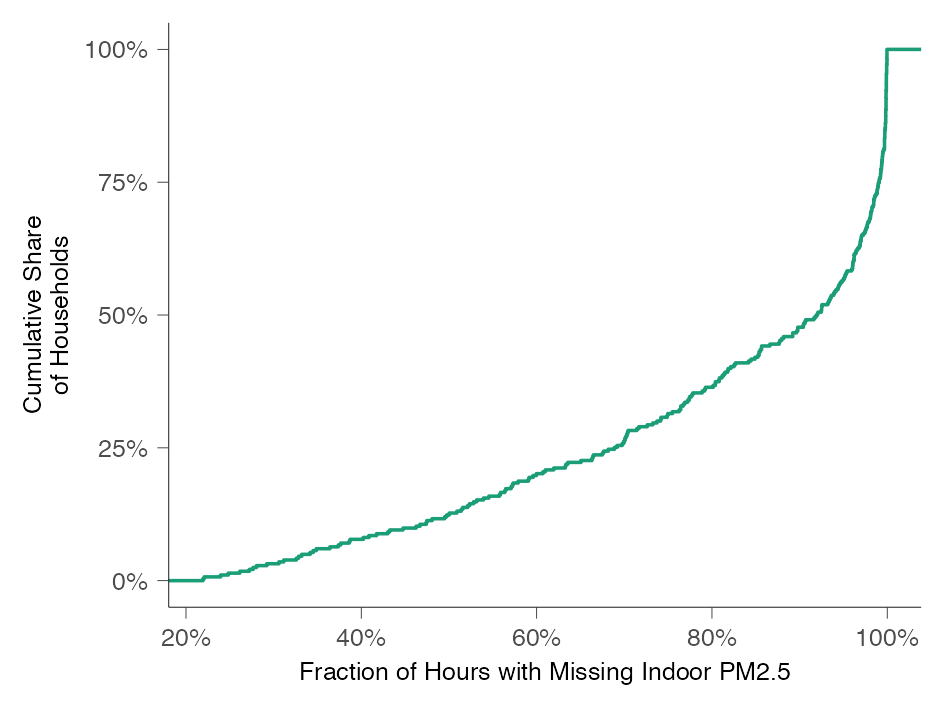
\includegraphics[width=.6\linewidth]{output_clean/figures/fig_appendix_missing_data.png}
    \caption*{\footnotesize Notes: Empirical cumulative distribution function of missing indoor PM$_{2.5}$ data. Each observation represents a household; the x-axis shows the fraction of that household's hourly PM$_{2.5}$ readings that are missing, and the y-axis shows the cumulative share of households at or below that fraction.}
    \label{fig:indoor_missing}
\end{figure}
\vfill
\clearpage


\pagebreak
\begin{figure}[!h] %3
    \centering
    \caption{Infiltration Factor With Varying Weights} 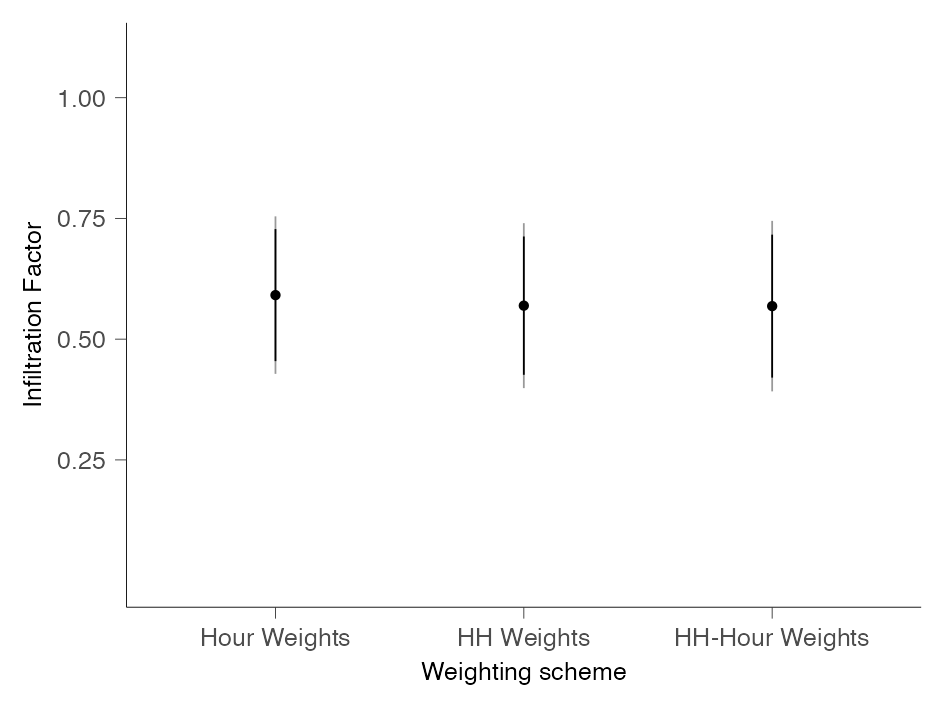
\includegraphics[width=.6\linewidth]{output_clean/figures/fig_appendix_inf_by_weight.png}
    \caption*{\footnotesize Notes: Each column reports the coefficient on outdoor PM$_{2.5}$ (the infiltration factor) from estimating the main infiltration specification. Column 1 is our main specification, which does not have any weights. This implicitly upweights households with more available data. Column 2 weights by the inverse of the household-specific observation rate, upweighting households with more missing data. Column 3 weights by the inverse of the household-by-hour observation rate, upweighting household-hour cells with more missing data. Observation rates are defined as the fraction of non-missing indoor PM$_{2.5}$ readings within the relevant grouping. Darker error bars show 90\% confidence intervals, and lighter error bars show 95\% confidence intervals. Standard errors are clustered at the household and date-hour level.}
    \label{fig:dist_sensor}
\end{figure} 


\pagebreak
\vfill
\centering
\begin{figure}[!h]%2
    \centering
    \caption{Infiltration Factor at Varying Distance to Outdoor Sensor} 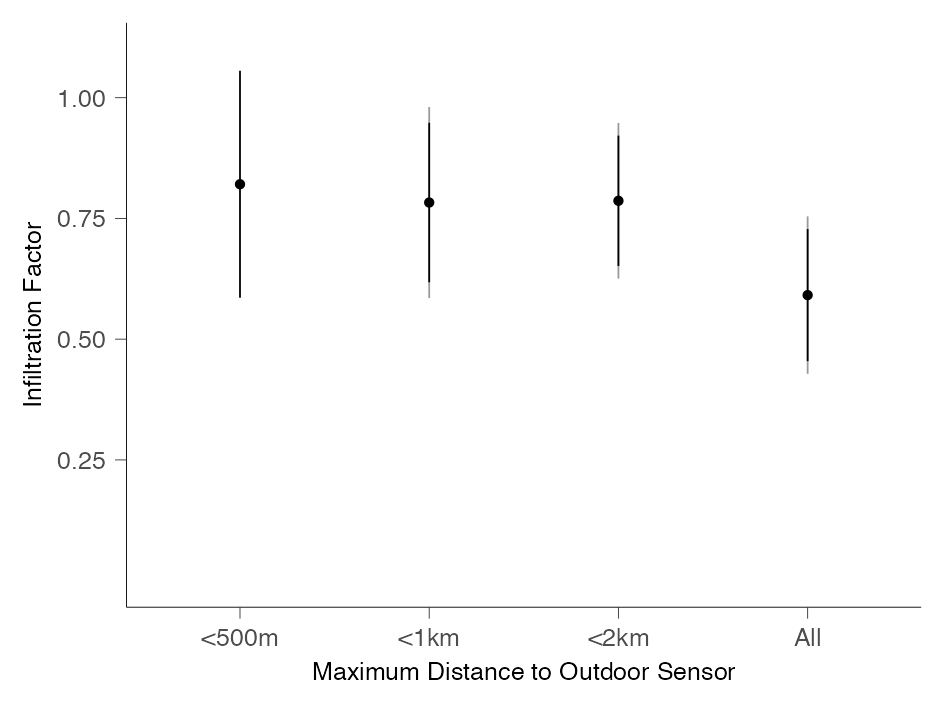
\includegraphics[width=.6\linewidth]{output_clean/figures/fig_appendix_inf_by_distance.png}
    \caption*{\footnotesize Notes: Each point reports the coefficient on outdoor PM$_{2.5}$ (the infiltration factor) from estimating Equation 1 with hour-of-day and week fixed effects, controlling for hyperlocal source variables, outdoor temperature, and humidity. The sample is progressively restricted to households located within 0.5km, 1km, and 2~km of the nearest outdoor air quality sensor; the rightmost point uses the full sample with no distance restriction. Darker error bars show 90\% confidence intervals, and lighter error bars show 95\% confidence intervals. Standard errors are clustered at the household and date-hour level.}
    \label{fig:dist_sensor}
\end{figure} 
\vfill

x
\vfill
\centering
\begin{figure}[!h]%2
    \centering
    \caption{Infiltration Factor at Varying Ambient Outdoor Temperatures} 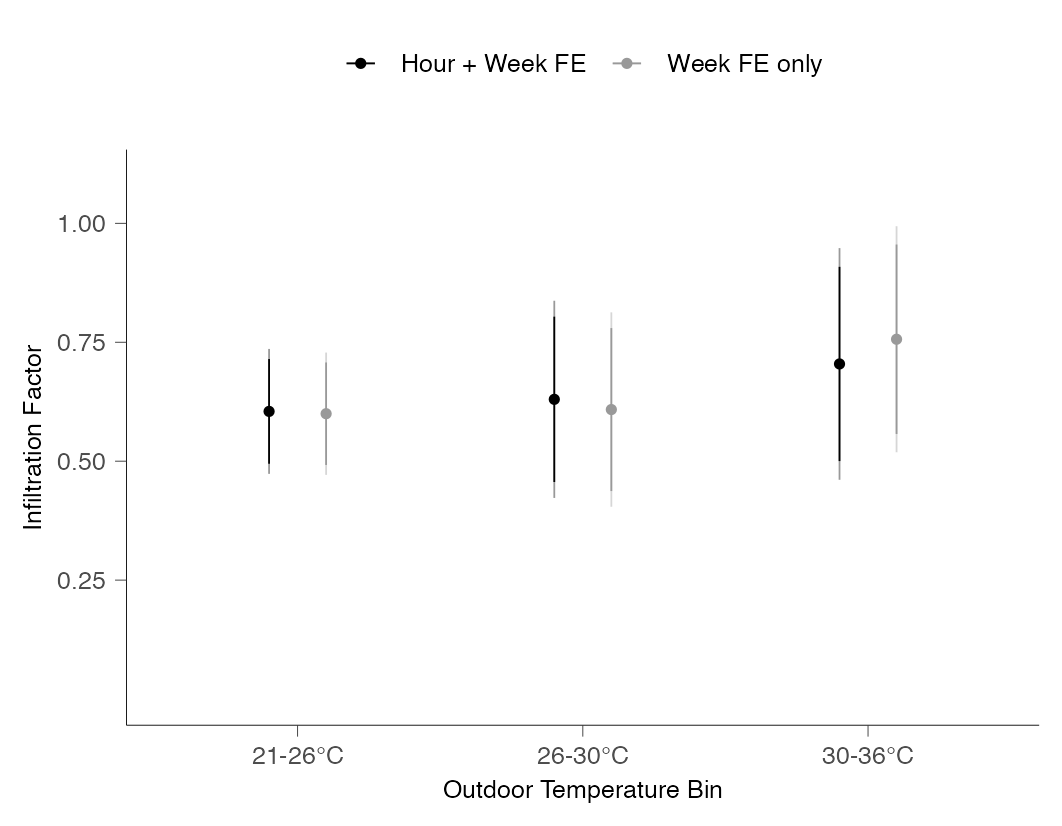
\includegraphics[width=.6\linewidth]{output_clean/figures/fig_appendix_inf_by_temp.png}
    \caption*{\footnotesize Notes: Each black point reports the coefficient on outdoor PM$_{2.5}$ (the infiltration factor) from estimating Equation 1 with hour-of-day and week fixed effects, controlling for hyperlocal source variables and humidity. Each grey point reports the coefficient on outdoor PM$_{2.5}$ (the infiltration factor) from estimating Equation 1 but without hour-of-day fixed effects. The sample is successively restricted to observations with outdoor temperature between 21-26$^o$C, 26-30$^o$C, and 30-36$^o$C. Darker error bars show 90\% confidence intervals, and lighter error bars show 95\% confidence intervals. Standard errors are clustered at the household and date-hour level.}
    \label{fig:temp}
\end{figure} 
\vfill


\newpage
\begin{figure}[!htb] %7
    \centering
    \caption{Source Contributions to PM$_{2.5}$ Spikes} 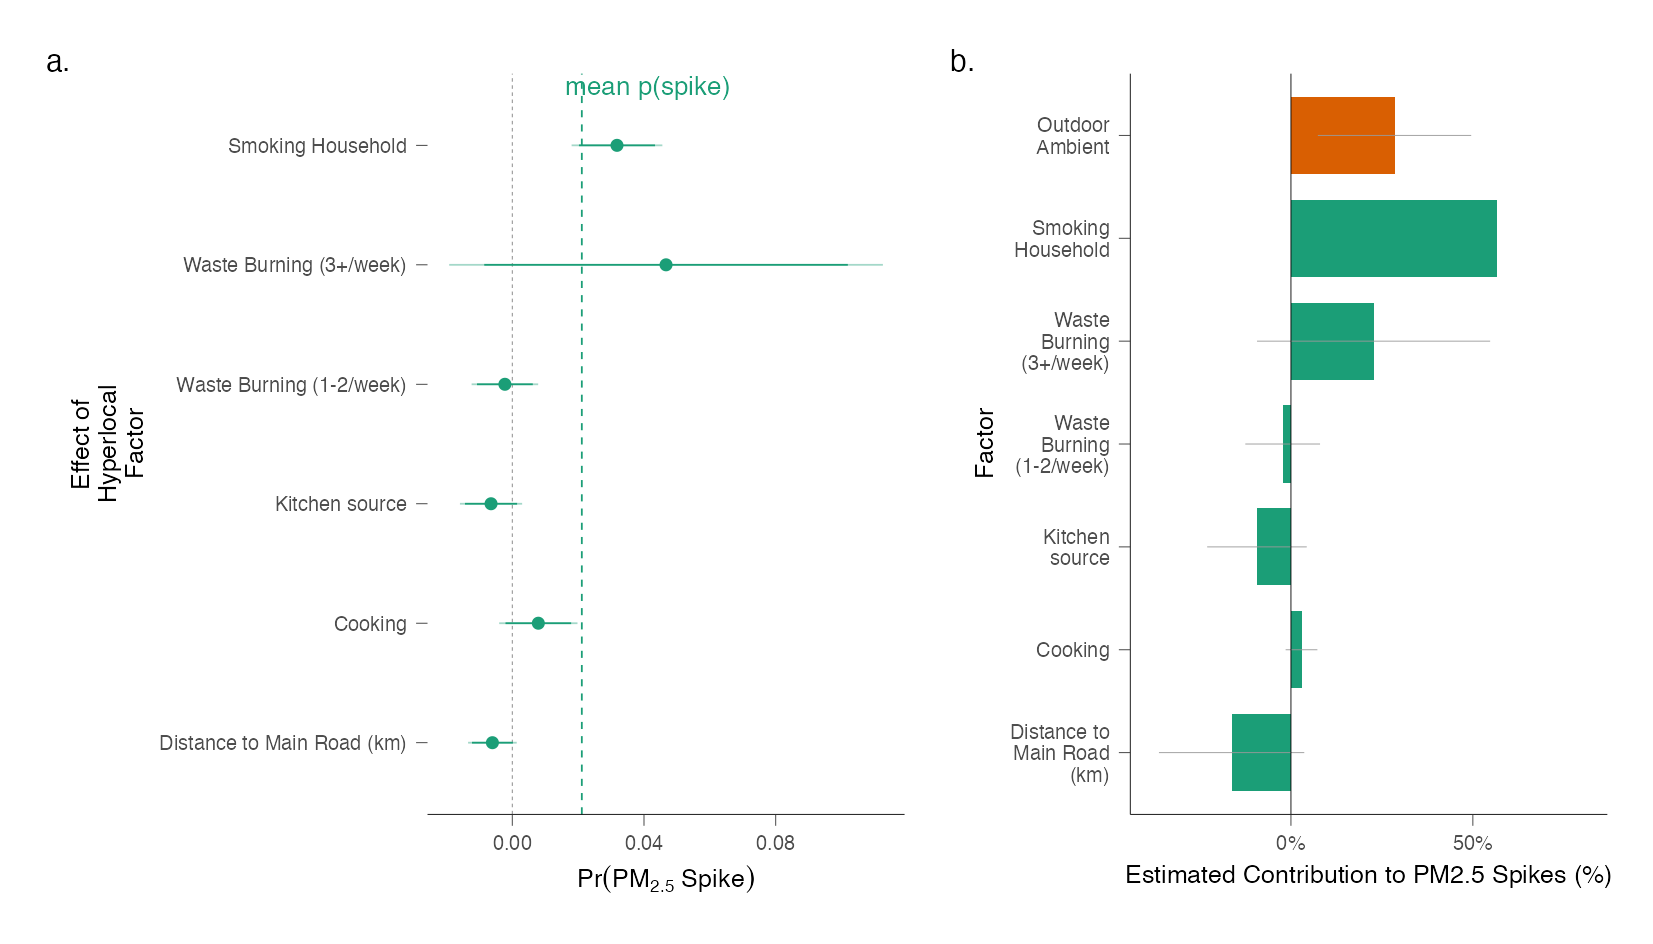
\includegraphics[width=\linewidth]{output_clean/figures/fig_appendix_spike_sources.png} 
    \caption*{\footnotesize Notes: Analogous to Figure 3 but with PM$_{2.5}$ spikes as the outcome variable. Spikes are defined as hours in which the hour-to-hour change in indoor PM$_{2.5}$ exceeds one standard deviation of the overall indoor PM$_{2.5}$ distribution. (a) Coefficient estimates from estimating Eq. (1) with the spike indicator as the dependent variable. The dashed green line indicates the sample mean spike probability. (b) Estimated mean contribution of each source to PM$_{2.5}$ spikes, calculated by multiplying each regression coefficient by the sample mean of its corresponding variable and expressing the product as a share of the mean spike probability. Error bars reflect 95\% confidence intervals, computed by scaling the upper and lower bounds of each coefficient's confidence interval by the corresponding sample mean. Standard errors are clustered at the household and date-hour level. }
    \label{fig:spikes}
\end{figure}

\newpage

\begin{figure}[!htb] %6
    \centering
    \caption{CDF of household distance to roads} 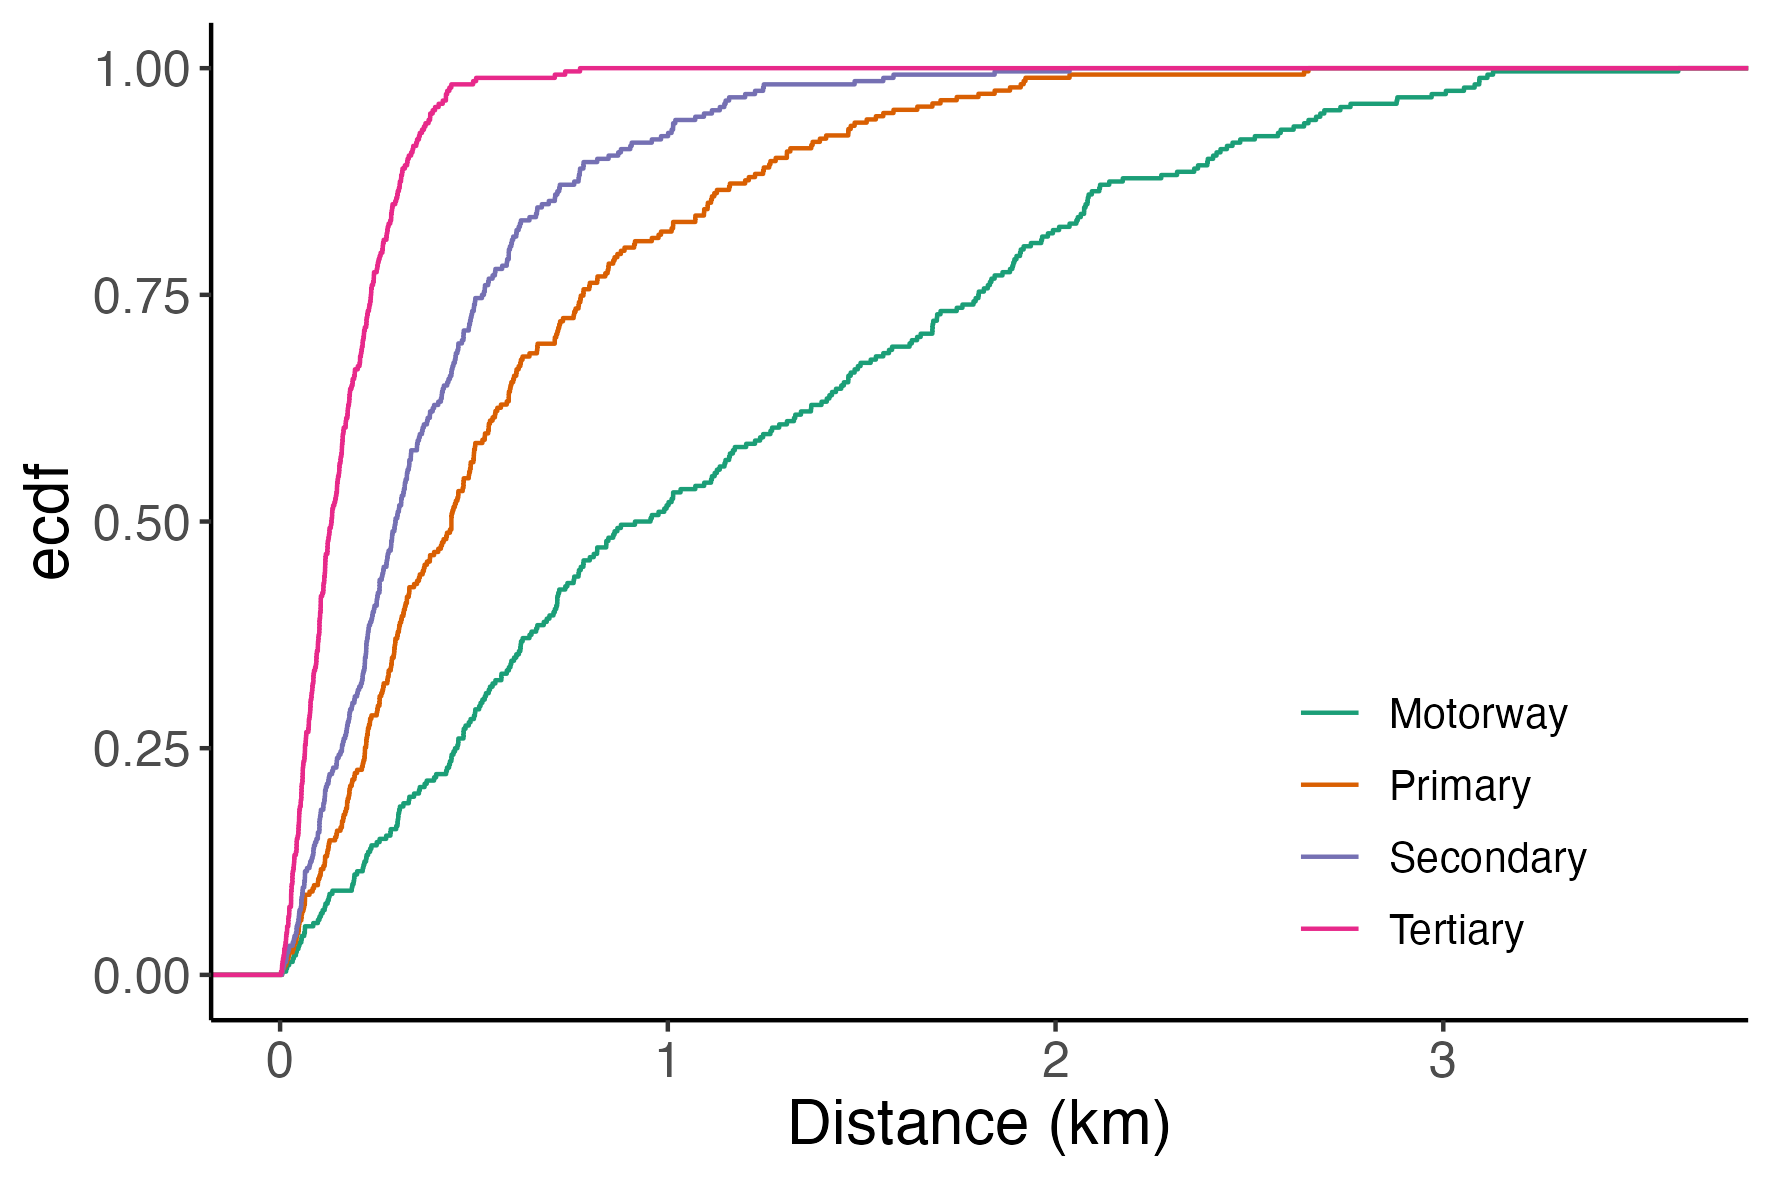
\includegraphics[width=.6\linewidth]{output_clean/figures/distance_to_road_ecdf.png}
    \caption*{\footnotesize Notes: This figure shows the cumulative distribution of each household's distance to the nearest road, by road type. Motorways are limited-access highways or toll roads, primary roads are major arterial roads connecting districts and cities, secondary roads are collector roads connecting neighborhoods, and tertiary roads are local residential streets.}
    \label{fig:inf_lag}
\end{figure}


\pagebreak
\begin{figure}[!htb] %5
    \centering
    \caption{Robustness: Mean $PM_{2.5}$ Under Various Aggregation Methods} 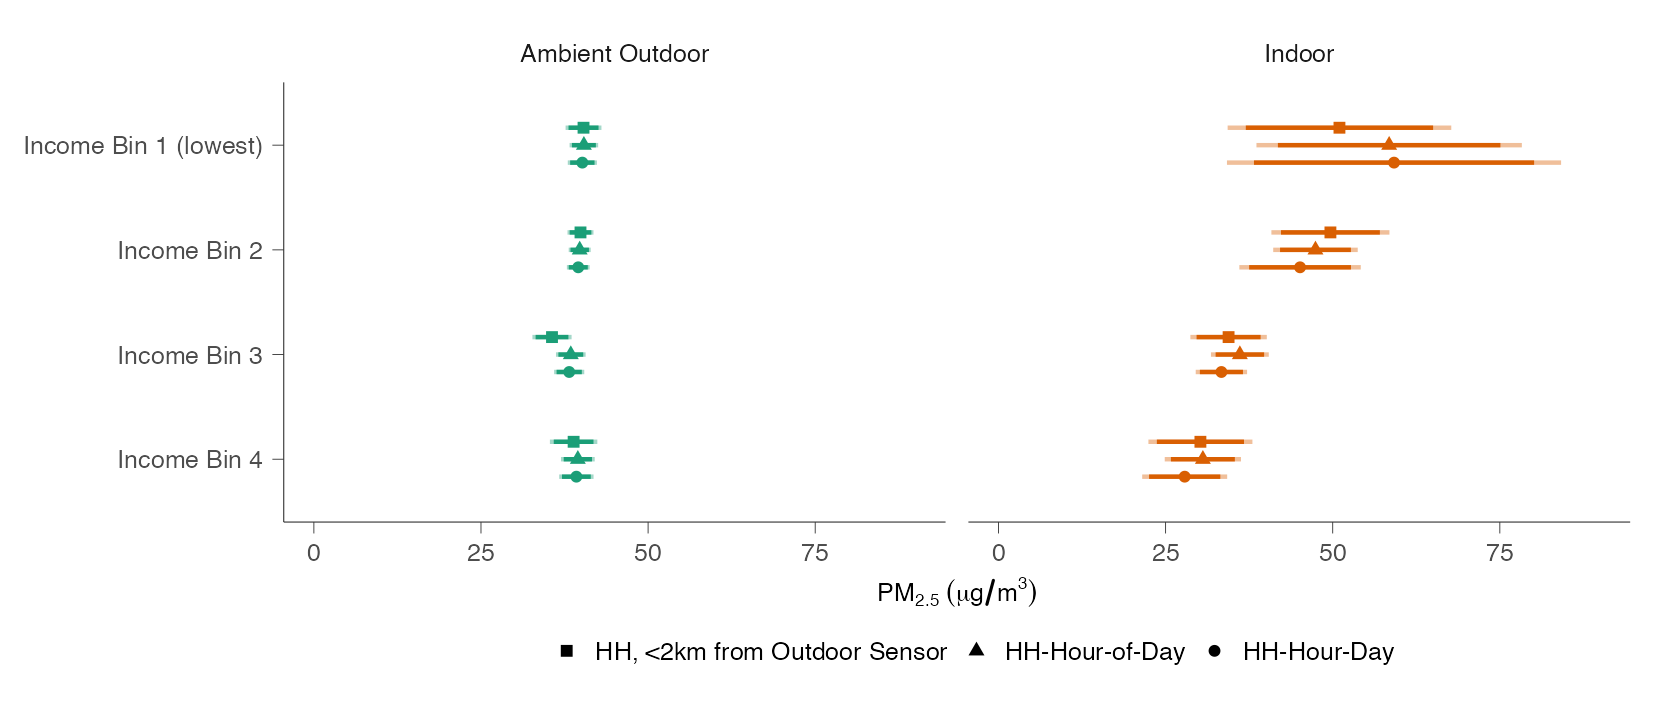
\includegraphics[width=\linewidth]{output_clean/figures/pm_income_robustness.png}
    \caption*{\footnotesize Notes: Mean outdoor ambient (left) and indoor (right) $PM_{2.5}$ concentrations across income quartiles, aggregated using three different methods to show robustness. \textit{HH, $<2$km from Outdoor Sensor}, calculates a single mean \( PM_{2.5} \) value per household, restricting the sample to households located within 2 km of an outdoor sensor to ensure proximity-based comparability. \textit{HH-Hour-of-Day}, aggregates data by computing the mean \( PM_{2.5} \) concentration for each household at each hour of the day. \textit{HH-Hour-Day} uses mean \( PM_{2.5} \) concentrations at the level of each household-hour-date. These mean $PM_{2.5}$ are then regressed onto the income quartile. Points represent mean estimates; darker error bars show 90\% confidence intervals, and lighter error bars show 95\% confidence intervals. Errors are clustered at the household level.
 }
    \label{fig:pm_income_robust}
\end{figure}

\pagebreak


\begin{figure}[!htb]
    \centering
    \caption{Sensor validation} 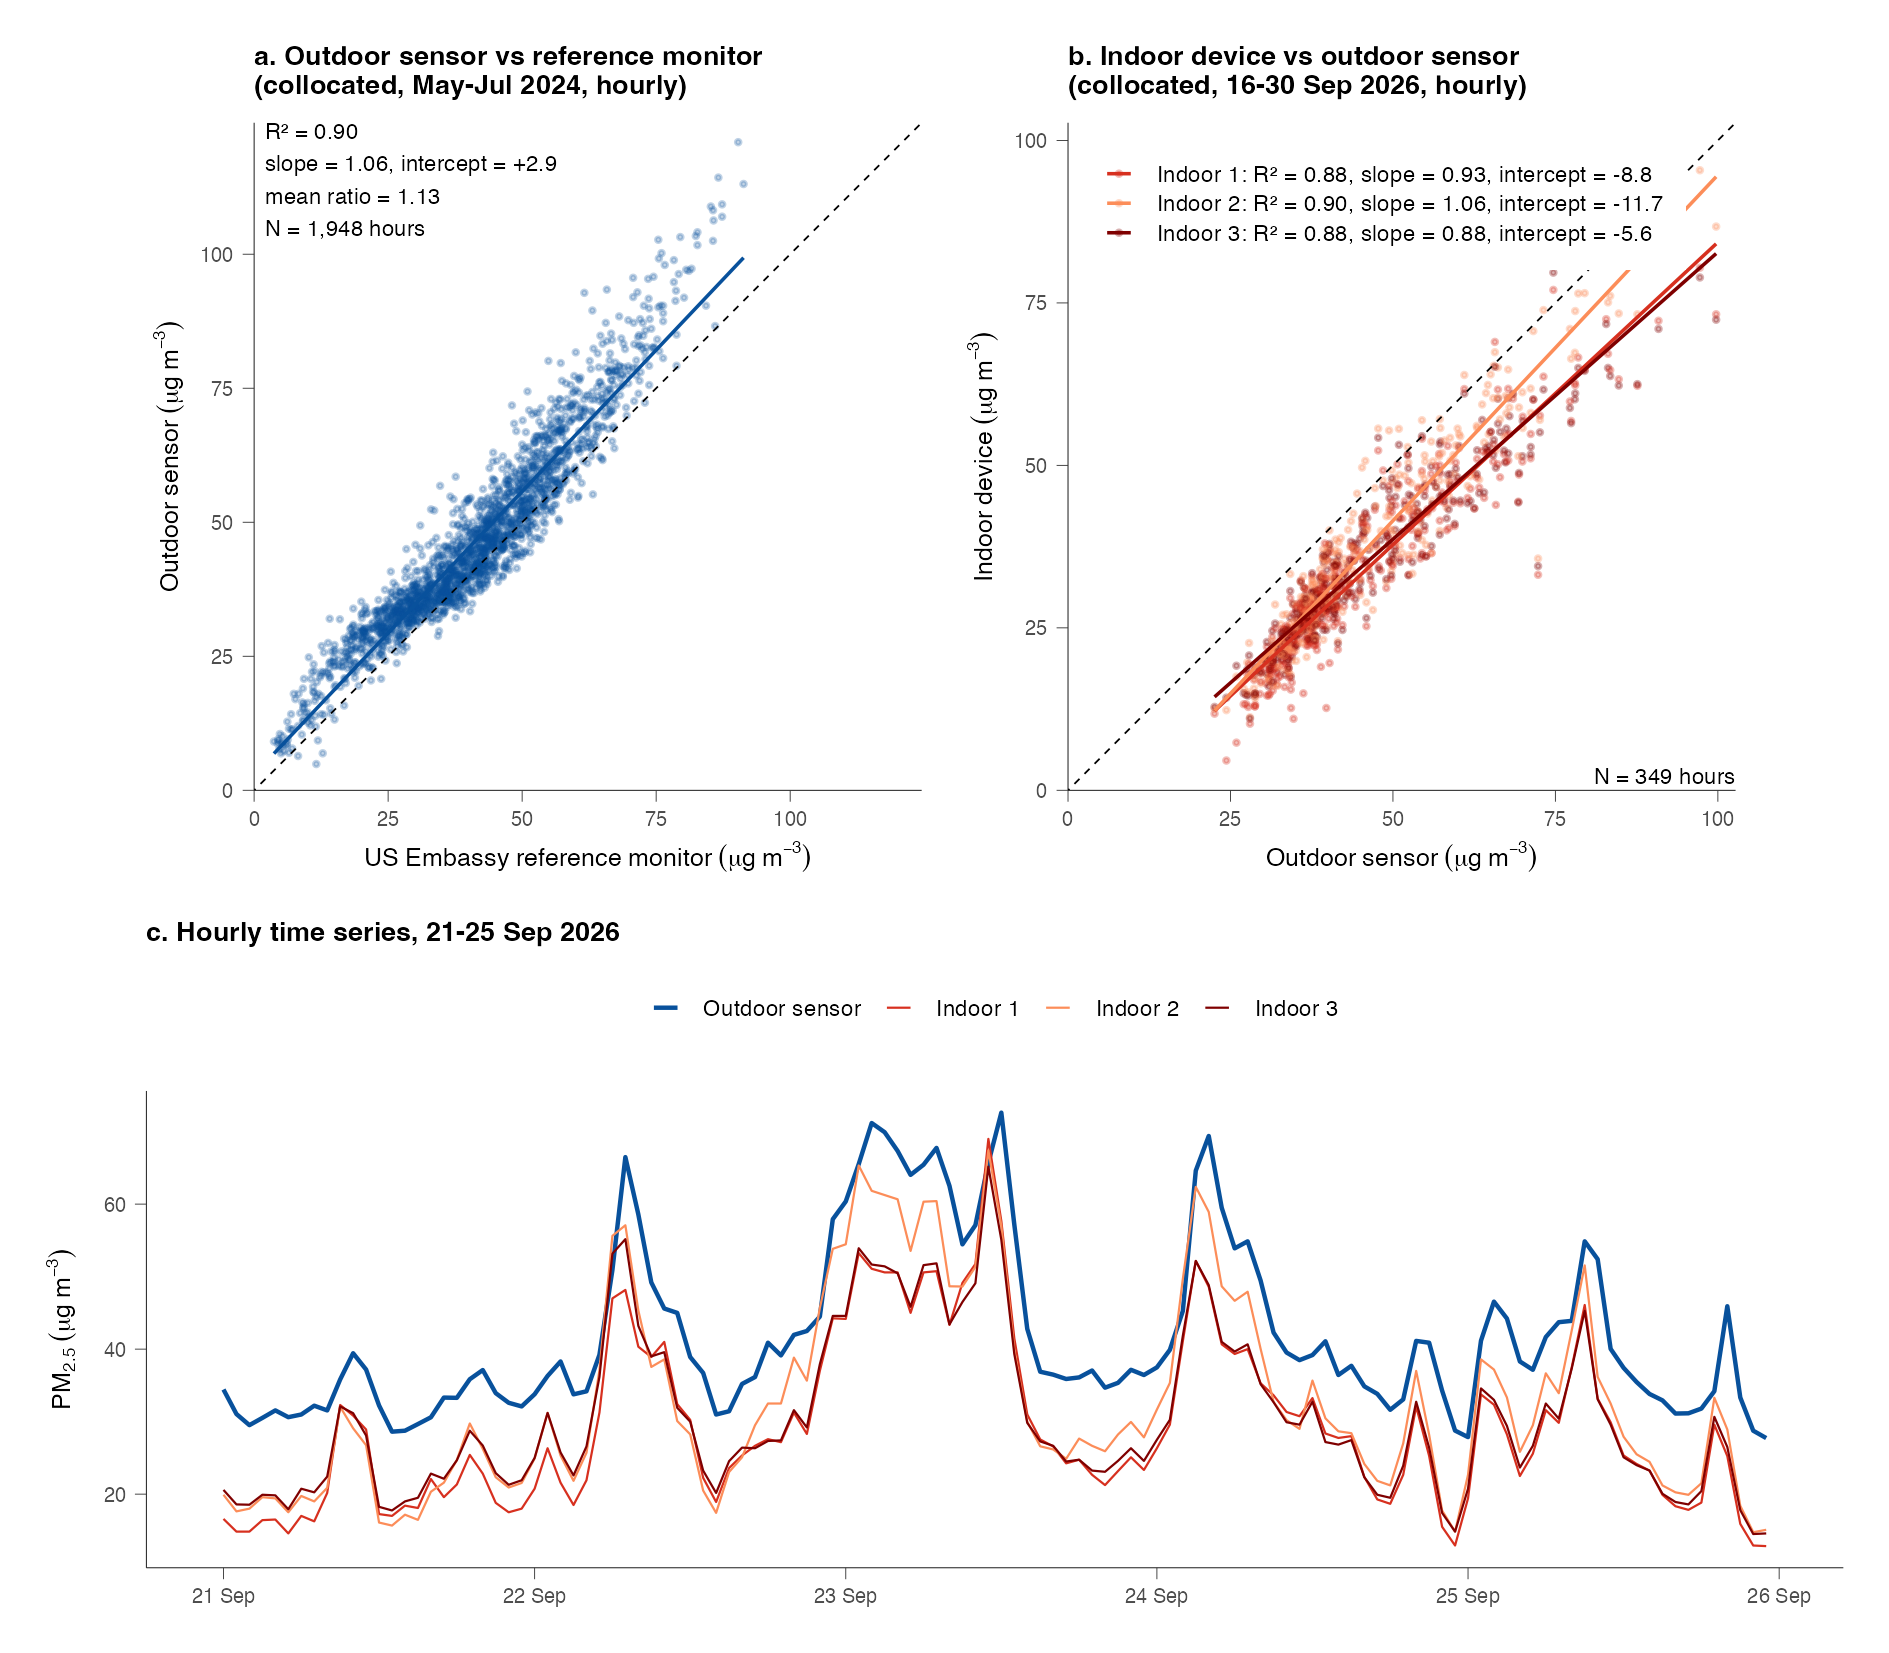
\includegraphics[width=\linewidth]{output_clean/figures/figS_sensor_validation.png}
    \caption*{\footnotesize Notes: (a) Hourly PM$_{2.5}$ from an Airly outdoor sensor (Plantower PMS5003) against a collocated US Embassy reference monitor, May--July 2024. (b) Hourly PM$_{2.5}$ from three indoor devices (Cubic PM2008M) against a collocated Airly outdoor sensor (Plantower PMS5003), 16--30 September 2026. We exclude the first day, during which the devices were warming up, and a short local pollution spike from waste burning on 26 September (05:00--07:59) that saturated the instruments. (c) Hourly time series from panel b, 21--25 September 2026. In each scatter plot, dashed lines show the 1:1 line and solid lines OLS fits.}
    \label{fig:sensor_validation}
\end{figure}



\pagebreak

\newpage
\section*{Tables}



\begin{table}[!h] %1
    \centering

    \caption{\textbf{Source Contribution to Mean Indoor PM$_{2.5}$}}
    \label{tab:source}
    \begin{adjustbox}{max width=\textwidth}
    \small
    
\begin{tabular}{cccccc}
\toprule
Source & Reg. Estimate & p.value & Mean Value of Source & Mean Contribution & $R^2$ Contribution\\
\midrule
Outdoor Ambient & 0.59 & 0.000 & 39.41 & 56\% & 33\%\\
Smoked (24 Hours) & 21.33 & 0.001 & 0.38 & 19\% & 23\%\\
Kitchen source & -0.28 & 0.968 & 0.31 & 0\% & 0\%\\
Cooking & -2.49 & 0.469 & 0.08 & 0\% & 0\%\\
Distance to Main Road (km) & 3.52 & 0.707 & 0.57 & 5\% & 0\%\\
\addlinespace
Waste Burning (1-2/week) & -1.76 & 0.743 & 0.21 & -1\% & \\
Waste Burning (3+/week) & 46.85 & 0.168 & 0.10 & 12\% & \\
\bottomrule
\end{tabular}

    \end{adjustbox}
    \caption*{\footnotesize \textit{Notes:} Regression estimates are from Figure 3a, a fixed-effects model of hourly indoor PM$_{2.5}$ on source variables with hour-of-day and week fixed effects; standard errors are clustered at the household and date-hour level. ``Reg. Estimate" reports the coefficient on each source. "Mean Value of Source" is the sample mean of the corresponding variable (Figure 3b). ``Mean Contribution" is the product of the coefficient and the sample mean, expressed as a share of mean indoor PM$_{2.5}$. ``$R^2$ Contribution" reports the proportional contribution of each source to explained variance using the Lindeman-Merenda-Gold (LMG) decomposition from a linear model with hour and week indicators. The LMG decomposition aggregates across levels of categorical variables (e.g., waste burning frequencies), so a single $R^2$ contribution is reported for waste burning overall.}
\end{table}

\newpage

\begin{table}[!h] %2
    \centering

    \caption{\textbf{Association Between Reported Waste Burning and Outdoor PM$_{2.5}$}}
    \label{tab:waste}
    \begin{adjustbox}{max width=.7\textwidth}
    \small
    
\begin{tabular}{lcc}
   \toprule
   Dependent Variable: & \multicolumn{2}{c}{Outdoor PM2.5}\\
                            & Closest 3 Sensors & HH Within 2km of Outdoor Sensor \\   
   Model:                   & (1)               & (2)\\  
   \midrule
   \emph{Variables}\\
   Waste Burning (1-2/week) & 0.570             & 0.431\\   
                            & (0.779)           & (0.770)\\   
   Waste Burning (3+/week)  & 4.06$^{***}$      & 5.12$^{***}$\\   
                            & (1.06)            & (1.79)\\   
   Outdoor Temperature      & -0.351            & 0.182\\   
                            & (0.248)           & (0.260)\\   
   Outdoor Humidity         & -0.182$^{***}$    & -0.164$^{***}$\\   
                            & (0.043)           & (0.048)\\   
   \midrule
   \emph{Fixed-effects}\\
   Week FE                  & Yes               & Yes\\  
   Hour FE                  & Yes               & Yes\\  
   \midrule
   \emph{Fit statistics}\\
   Observations             & 759,777           & 394,345\\  
   R$^2$                    & 0.38432           & 0.37470\\  
   Within R$^2$             & 0.00992           & 0.01250\\  
   \bottomrule
\end{tabular}



    \end{adjustbox}
    \caption*{\footnotesize \textit{Notes:}  Each column regresses outdoor PM$_{2.5}$ on household-reported waste burning frequency in the neighborhood over the preceding 7 days, controlling for outdoor temperature and humidity, with hour-of-day and week fixed effects. Column 1 assigns each household the mean PM$_{2.5}$ reading from the three nearest government sensors. Column 2 restricts the sample to households located within 2 km of an outdoor sensor. Clustered (respondent and date-hour FE) standard errors are in parentheses. Signif. Codes: $^{***}$: 0.01, $^{**}$: 0.05, $^{*}$: 0.1.}
\end{table}

\newpage

\begin{table}[!h] %3
    \centering

    \caption{\textbf{Source Contribution to Spikes in Indoor PM$_{2.5}$}}
    \label{tab:spike_source}
    \begin{adjustbox}{max width=\textwidth}
    \small
    
\begin{tabular}{cccccc}
\toprule
Source & Reg. Estimate & p.value & Mean Value of Source & Mean Contribution & $R^2$ Contribution\\
\midrule
Outdoor Ambient & 0.000 & 0.008 & 39.41 & 28\% & 2\%\\
Smoking Household & 0.032 & 0.000 & 0.38 & 57\% & 54\%\\
Kitchen source & -0.006 & 0.180 & 0.31 & -9\% & 2\%\\
Cooking & 0.008 & 0.191 & 0.08 & 3\% & 1\%\\
Distance to Main Road (km) & -0.006 & 0.109 & 0.57 & -16\% & 5\%\\
\addlinespace
Waste Burning (1-2/week) & -0.002 & 0.663 & 0.21 & -2\% & \\
Waste Burning (3+/week) & 0.047 & 0.164 & 0.10 & 23\% & \\
 &  &  &  &  & 19\%\\
\bottomrule
\end{tabular}

    \end{adjustbox}
    \caption*{\footnotesize \textit{Notes:} Estimates  from a fixed-effects regression of a binary spike indicator on source variables, with hour-of-day and week fixed effects; standard errors are clustered at the household and date-hour levels. A spike is defined as an hourly PM$_{2.5}$ reading that exceeds the preceding hour by at least one standard deviation.  ``Reg. Estimate" reports the coefficient on each source (from Figure S6). ``Mean Value of Source" is the sample mean of the corresponding variable. ``Mean Contribution" is the product of the coefficient and the sample mean, expressed as a share of PM$_{2.5}$ spike probability. ``$R^2$ Contribution" reports the proportional contribution of each source to explained variance using the Lindeman-Merenda-Gold (LMG) decomposition from a linear model with hour and week indicators. The LMG decomposition aggregates across levels of categorical variables (e.g., waste burning frequencies), so a single $R^2$ contribution is reported for waste burning overall.}
\end{table}

\pagebreak 
\newpage

\begin{table}[!h] %4
    \centering

    \caption{\textbf{Back-of-the-envelope calculations of the effect of weatherization (reducing $a$) and reduced particle penetration of incoming air (reducing $P$) on indoor PM$_{2.5}$ concentrations.}}
    \label{SI_BoE_table}
    \begin{adjustbox}{max width=0.9\textwidth}
    \small
    % -----------------------------------------------------------------------
% Auto-generated by table_boe.R -- do not edit by hand
% -----------------------------------------------------------------------

\begin{tabular*}{\linewidth}{@{\extracolsep{\fill}}lccccc}
\toprule
%---- Panel A -------------------------------------------------------
\multicolumn{6}{l}{\textbf{Panel A. Data inputs and derived parameters}} \\[2pt]
  & $C_{in}$
  & $C_{out}$
  & $\hat{F}_{inf}$
  & $a$
  & $S$
  \\
  & ($\mu$g\,m$^{-3}$)
  & ($\mu$g\,m$^{-3}$)
  &
  & (h$^{-1}$)
  & ($\mu$g\,m$^{-3}$\,h$^{-1}$)
  \\
\cmidrule(lr){2-3}\cmidrule(lr){4-4}\cmidrule(lr){5-6}
Income Bin 1, Non-smoking & 49.0 & 40.0 & 0.593 & 0.7 & 31.0 \\
Income Bin 1, Smoking & 57.3 & 40.5 & 0.593 & 0.7 & 41.0 \\
Income Bin 4, Non-smoking & 28.2 & 40.0 & 0.551 & 0.6 & 6.9 \\
Income Bin 4, Smoking & 36.8 & 38.4 & 0.551 & 0.6 & 17.4 \\
\midrule
%---- Panel B -------------------------------------------------------
\multicolumn{6}{l}{\textbf{Panel B. Counterfactual $\Delta C_{in}$ ($\mu$g\,m$^{-3}$)}} \\[2pt]
  &
  \multicolumn{2}{c}{Weatherization ($a \times 0.8$)}
  &
  \multicolumn{2}{c}{Reduced Particle Penetration ($P \times 0.8$)}
  & \\
\cmidrule(lr){2-3}\cmidrule(lr){4-5}
  & Central
  & Robust.~range\textsuperscript{(a)}
  & Central
  & Direction
  & \\
\cmidrule(lr){2-3}\cmidrule(lr){4-5}
Income Bin 1, Non-smoking & $+1.2$ & [$+1.2$,\;$+2.9$] & $-4.7$ & Always $\downarrow$ & \\
Income Bin 1, Smoking & $+2.3$ & [$+2.3$,\;$+4.3$] & $-4.8$ & Always $\downarrow$ & \\
Income Bin 4, Non-smoking & $-1.5$ & [$-1.5$,\;$-0.6$] & $-4.4$ & Always $\downarrow$ & \\
Income Bin 4, Smoking & $-0.2$ & [$-0.2$,\;$+1.0$] & $-4.2$ & Always $\downarrow$ & \\
\bottomrule
\end{tabular*}

    \end{adjustbox}
    \caption*{\footnotesize \textit{Notes:} Panel A reports group means of $C_{in}$ and $C_{out}$ and the estimated infiltration factors $\hat F_{inf}$ by income group. Panel B reports counterfactual changes in indoor PM$_{2.5}$, $\Delta C_{in}$, relative to observed baseline concentrations from (i) weatherization modeled as $a \rightarrow 0.8a$ and (ii) reduced particle penetration of incoming air modeled as $P \rightarrow 0.8P$. \textsuperscript{(a)} Robust range varies $k \in [0.2,1.5]~h^{-1}$ and $P \in [0.8,1.0]$, recomputing $a=\frac{\hat F_{inf}k}{P-\hat F_{inf}}$ and $S=(C_{in}-\hat F_{inf}C_{out})(a+k)$ for each parameter setting as described in the text; the reported interval gives the minimum and maximum counterfactual $\Delta C_{in}$ across these settings.}
\end{table}

\newpage
% \setcounter{table}{0}
% \renewcommand{\thetable}{A\arabic{table}}

\begin{table}[!h] %5
    \centering

    \caption{\textbf{Summary Statistics of Household Survey}}
    \label{tab:covariates}
    \begin{adjustbox}{max width=.7\textwidth}
    \small
    
\begin{tabular}{lccc}
\toprule
Variable & Sample Mean & N & Population Mean\\
\midrule
Female & 0.9 & 283 & \\
 &  &  \vphantom{3} & \\
Age & 41.21 & 283 & \\
 & (6.91) &  & \\
HH Size & 5.13 & 283 & 3.79\\
 & (1.94) &  & (1.31)\\
Number of Children & 2.05 & 283 & \\
 & (1.03) &  & \\
HH Monthly Exp. (USD) & 248.74 & 275 & 655.94\\
 & (117.16) &  & (707.71)\\
HH Monthly Income (USD) & 312.48 & 281 & \\
 & (194.17) &  & \\
HH Head Attended Secondary & 0.88 & 283 & 0.88\\
 &  &  \vphantom{2} & \\
HH Head Attended Tertiary & 0.14 & 283 & 0.3\\
 &  &  \vphantom{1} & \\
Owns AC & 0.55 & 282 & 0.39\\
 & (0.5) &  & \\
LPG Stove & 0.98 & 283 & 0.96\\
 &  &  & \\
Number of Smokers & 0.93 & 283 & 0.73\\
 & (0.85) &  & (0.71)\\
\midrule
\bottomrule
\end{tabular}

    \end{adjustbox}
    \caption*{\footnotesize \textit{Notes:}  Household characteristics and comparisons to the Jakarta population mean. Population means were calculated using data from the National Socioeconomic Survey (SUSENAS) 2023.}
\end{table}


\begin{table}[!h] %6

    \centering

    \caption{\textbf{Distance to Outdoor Sensor Not Correlated with Household Characteristics}}
    \label{tab:sensor_selection}
    \begin{adjustbox}{max width=.7\textwidth}
    \small
    
\begin{tabular}{lc}
   \toprule
   Dependent Variable:           & Distance to Outdoor Sensor (meters)\\  
   Model:                        & (1)\\  
   \midrule
   \emph{Variables}\\
   Indoor PM2.5                  & -0.99\\   
                                 & (2.44)\\   
   Outdoor PM2.5                 & 1.19\\   
                                 & (9.21)\\   
   Income (USD)                  & 0.13\\   
                                 & (0.58)\\   
   Housing Size                  & 42.52\\   
                                 & (53.36)\\   
   AC                            & -198.33\\   
                                 & (197.47)\\   
   HOH Employed                  & 314.69\\   
                                 & (374.62)\\   
   HOH Attended Secondary School & -285.71\\   
                                 & (305.55)\\   
   HOH Attended Tertiary School  & -173.15\\   
                                 & (317.86)\\   
   \midrule
   \emph{Fit statistics}\\
   Dependent variable mean       & 2,337.6\\  
   Observations                  & 283\\  
   \bottomrule
\end{tabular}



    \end{adjustbox}
    \caption*{\footnotesize \textit{Notes:} Regression of households' distance to nearest outdoor sensor on household covariates. IID standard-errors in parentheses. Signif. Codes: $^{***}$: 0.01, $^{**}$: 0.05, $^{*}$: 0.1.}
\end{table}






\pagebreak
\clearpage 
\bibliography{JakartaPM}
% \bibliography{pnas-sample}


\end{adjustwidth}
\end{document}